\chapter{Converting Vector Spaces into Interpretable Representations}\label{Chapter3}


\section{Introduction}\label{chapter3:Introduction}

% What is this chapter? What can I expect from this chapter?
This chapter describes how to go from a domain-specific Semantic Space (see Section \ref{bg:SemanticSpaces}) to producing linear classifiers driven by features where each dimension is a ranking on a distinct labelled property in the domain. By a property, we mean a semantically meaningful aspect of domain knowledge that entities can be ranked on. We show an example representation and classifier that were obtained from a Semantic Space constructed from IMDB movie reviews in figure \ref{ch3:TreeAndRep}.  We find that these representations are more interpretable than standard baseline interpretable representations (e.g. Topic Models), and also find that they outperform baseline harder to understand classifiers (Linear SVM's) in F1-score for some tasks, even when constrained to a very simple linear classifier. 

\begin{figure}[t]
	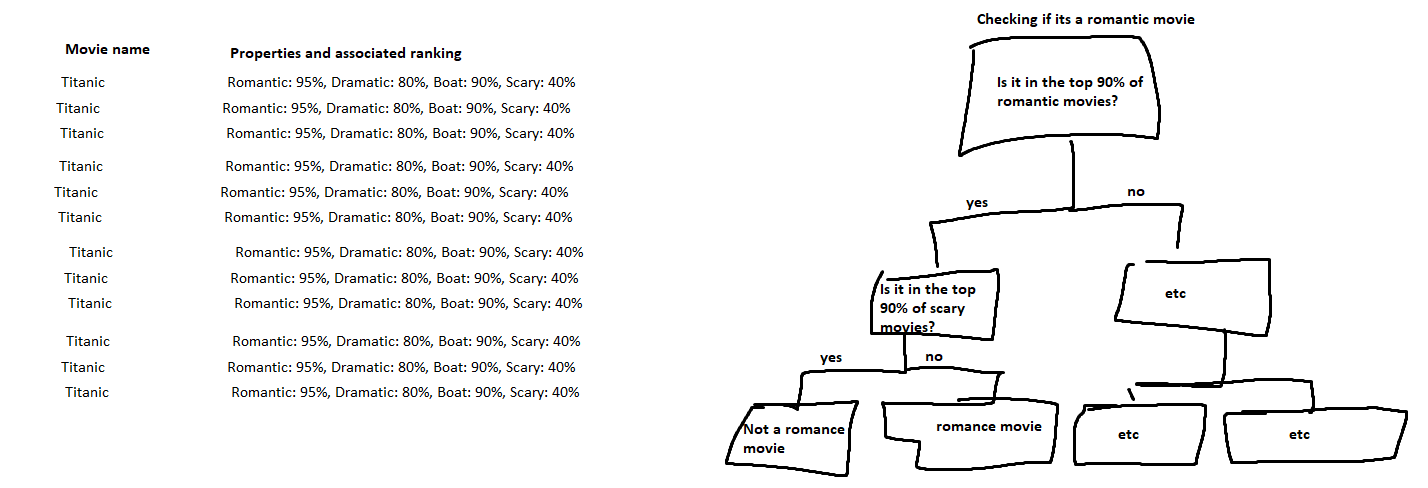
\includegraphics[width=\textwidth]{images/tree and rep.png}
	\centering
	\caption{Movies and selected associated dimensions, and their use in a linear classifier.}\label{ch3:TreeAndRep}
\end{figure}

\subsection{Semantic Relations}

%Semantic spaces encode semantic relationships

%What are the applications of semantic relationships? What is the power of a semantic relationship? Why are semantic relationships important in a space?
The success of these semantic spaces similarity-based structure has lead many to investigate how to formalize the relationships they encode spatially. One such striking example is in that of linear analogies in word-vectors (see Section \ref{WordVectors}, where it was found that the vector XXXX[]King queen blah blah[]XXXXXXX, formally justified in \cite{Ethayarajh2018}. %Vector example
These relationships have been expanded on, for example \cite{TomasMikolovWen-tauYih2013} found that "equivalent relations tended to correspond to parallel vector differences" \cite{Mitchell2015}, while \cite{Mitchell2015} discovered that by decomposing representations into orthogonal semantic and syntactic subspaces they were able to produce substantial improvements on various tasks. Additionally, \cite{Garg2017} found that word distances between gendered words (e.g. male, female, she, her) and occupational words e.g. (nurse, programmer) were correlated to the percentage of occupation that gender had for that role in different time periods. %Copy pasted from this 


%What are directions? Why are directions important? What have they been used for? What is a feature direction?
The semantic relation that we focus in on this paper are directions that correspond to salient features from the considered domain. A "direction" refers in this case to the orthogonal direction to a hyper plane that separates a term in a vector space. As the hyper plane separates entities, this means that the entities furthest along the hyper plane, at the end classified positively, are the entities we are most sure have the term we found the hyper plane for. To see an example of this, see \ref {LRHyperPlane} With this understanding, it becomes possible to induce a ranking of entities on the properties by finding the dot product of the entity points on the direction vector. These kind-of directions have been used in many different ways for different domains, For instance,  \cite{gupta2015distributional} found that features of countries, such as their GDP, fertility rate or even level of CO$_2$ emissions, can be predicted from word embeddings using a linear regression model. Similarly, in \cite{kim2013deriving} directions in word embeddings were found that correspond to adjectival scales (e.g.\ bad $<$ okay $<$ good $<$ excellent) while \cite{DBLP:conf/acl/RotheS16} found directions indicating lexical features such as the frequency of occurrence and polarity of words. 


\subsection{Producing an Interpretable Property Representation}

% How can I apply directions to produce an interpretable space? Why is this valuable? What makes this interesting? What are feature rankings?
By finding the dot product between entity points in the space and direction vectors, it is possible to induce a ranking of entities on those directions. In this chapter, we more deeply investigate the potential of direction vectors to rank entities on properties to form an interpretable representation.  In this thesis, we refer to these direction vectors as directions to convey the ordinal meaning, and directions as 'properties' if they are sufficiently salient in the space, e.g. In a domain of IMDB movie reviews where movies are entities, a direction on the word "The" would not be a property, but a direction on the word "Horror" would be. 

\begin{figure}[t]
	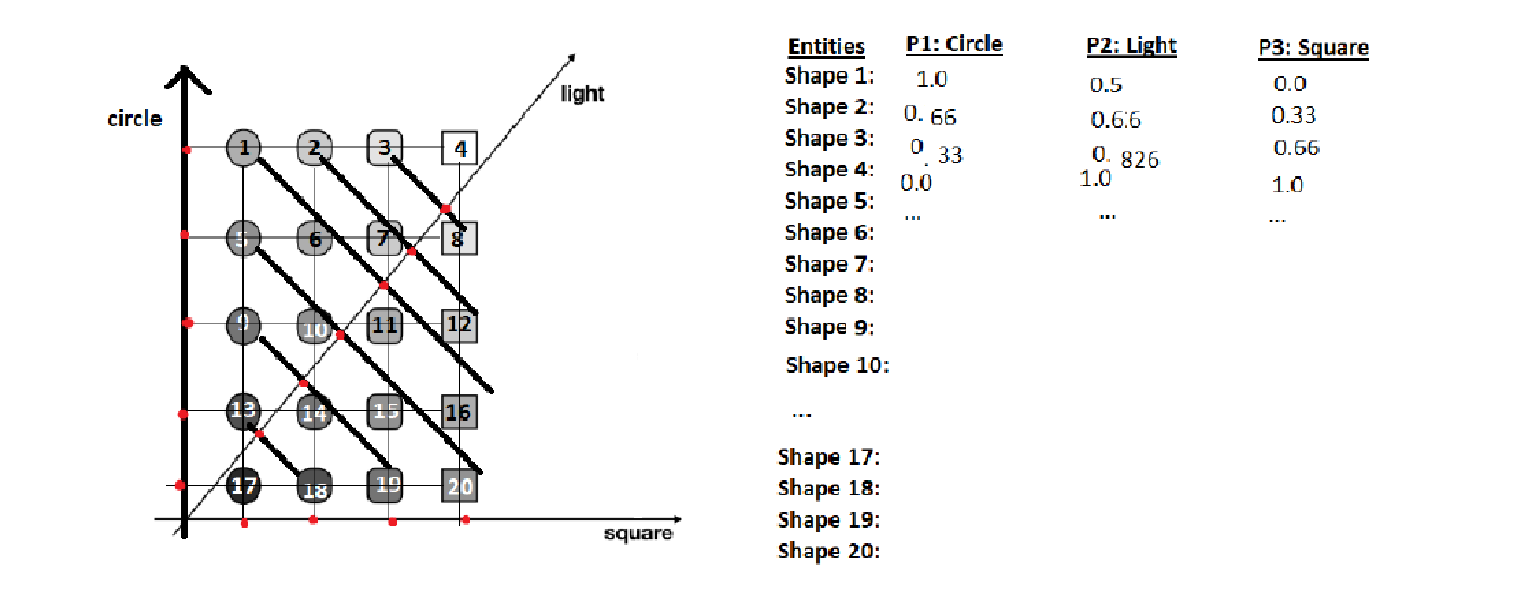
\includegraphics[width=\textwidth]{images/toydirections.png}
	\centering
	\caption{This figure shows a 2d toy space where entities are shapes and directions are properties. We demonstrate on the right the method to induce a ranking from the directions, in particular by using the dot-product of the entity point on the directions vector. In the same way for a more complex space, we can understand each entity point to be ranked on thousands of property directions, and the space to be much higher dimensionality.}\label{ToyDirection}
\end{figure}


%%What are the advantages, disadvantages of the previous work?

We demonstrate the effect of different filtering methods to find properties, the ability of different clustering methods to label properties, as well as the number and types of directions, for use in a low-depth interpretable linear classifier; a Decision Tree. In Figure \ref{IntroDecisionTree}, we demonstrate how depth could affect a Decision Tree that uses salient properties. These trees are not only evaluated quantitatively on key domain tasks, we also evaluate how interpretable the resulting rules are. This gives us a comprehensive idea of how we can use these rankings as an interpretable representation. By using a Decision Tree, we can identify salient properties - if we are able to construct a simple but high-scoring classifier for if a movie is a 'Comedy' using only our ranking of entities on the property $p = {"Funny", "Hilarious", "Laughing"}$ then we know that this property is salient. Although this is an extreme case, for more complex concepts, if we have salient properties that form the building blocks of this concept, then the model can be less complex and more general, two desirable properties for interpretable classifiers. 

\begin{figure}[t]
	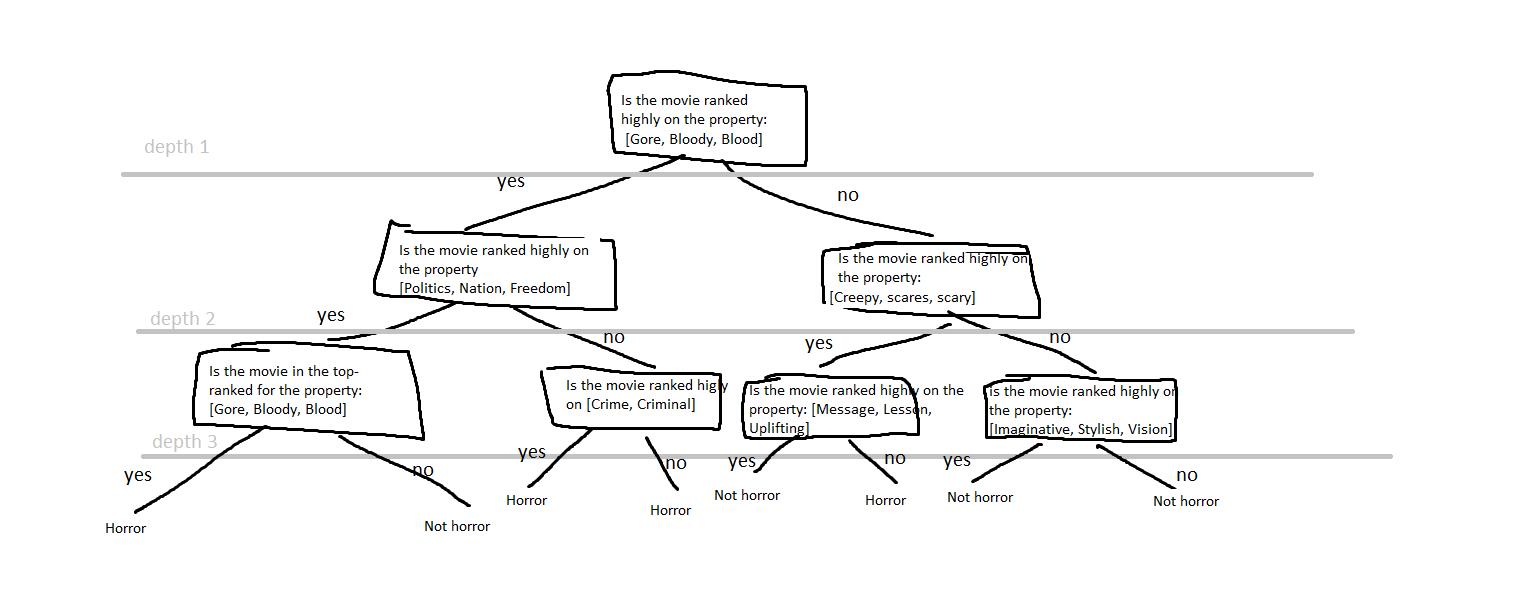
\includegraphics[width=\textwidth]{images/decisiontree.png}
	\centering
	\caption{This figure shows an example tree from one of our classifiers. Here, we can see that the model increases in complexity as it increases in depth. In this case, we end-up getting better F-score with just a depth-one tree, as the tree begins to overfit at depth three.  }\label{IntroDecisionTree}
\end{figure}

%Why do this work? What is the value of this work?  How is this relevant to the readers interests?


\subsection{Using a Property Representation in a Linear Classifier}


Our method can use any vector space that linearly separates entities, and so it has potential longevity.  This means that our method is relying on structure in the space that does not directly correspond to our desired representation -  we can view our approach as a linear transformation of the space. We address this problem in Chapter \ref{chapter:finetuning}. However, we have the capability to leverage many different methods to construct a vector space for our representation, so as long as dense representations of entities exist it will be possible to use our method, and as they are improved the results that our method can achieve will be improved too. This kind of flexibility also gives us the potential to combine the resultant representations from different vector spaces for classification, e.g. concatenating the vectors from different spaces.

Topic models such as Latent Dirichlet Allocation (LDA) represent documents as multinomial distributions over latent topics, where each of these topics corresponds to a multinomial distribution over words \cite{Blei2003}. These topics tend to correspond to semantically meaningful concepts, hence topic models tend to be rather interpretable \cite{Chang2009}. To characterize the semantic concepts associated with the learned topics, topics are typically labelled with the most probable words according to the corresponding distribution. 

% What is a semantic space? Why is a semantic space valuable?




% 





%%What is the previous work?
 %What is a direction




%Finally, \cite{derracAIJ} found salient properties as direction vectors in a semantic space of entities (e.g. Movies in a domain of IMDB movie reviews), and labelled them with clusters of words (e.g. $p_1 = {Scary, Horror, Gore}, p_2 = {Funny, Laughter, Hilarious}$).  We show a toy example in Figure \ref{ToyDirection}. %Copied from CONLL 




%%What is our contribution towards those disadvantages in this chapter?
 %"Decision Trees, Decision Tables and Textual descriptions of rules are logically equivalent in the sense that one type of representation can be automatically translated to another (albeit in a simpler or more complex form), while preserving the predictive behaviour of the original model"
% has many positive effects for its users, like lower response times \cite{Narayanan2018, Huysmans2011}, better question answering and confidence for logical problem questions \cite{Huysmans2011} and higher satisfaction \cite{Narayanan2018}.


%%What are some real world scenarios that you could see our work taking effect in?
%In a case study by  \cite{Veale2017}, giving the business users the option between a model with higher classification score but more input variables and a lower classification score but less input variables resulted in more buy-in for system designers. By accurately representing salient concepts in the domain, we are also able to offer a similar option; less nodes in the decision tree in exchange for more accuracy. % Potentially this citation sucks


%How is the work evaluated? How can you justify the evaluation? 
%%What are some alternative interpretable classifiers? What are some approaches to interpretable classification?

%%How does our work fit into the niche of interpretable classifiers?

%%What kind of tasks are these interpretable classifiers usually on? How do we compare in terms of evaluation?

%%How does our evaluation of interpretability play into our idea of interpretability outlined in Chapter 1?




%How is the chapter going to play out? Whats going to happen?

This chapter continues as follows: We begin by describing the work related to this , giving valuable context for the utility and potential of our approach. This is followed by an explanation of the method, including the variations we have adopted for our experimental work. We follow this with our qualitative experimentation, explaining how these variations affect the results, as well as the interpretability of the method, and we end with a quantitative analysis on how well we can represent domain knowledge using decision trees constrained to a limited depth.



\section{Related Work}
%Sparse word vectors
%Adapted to composition \cite{Fyshe2015}
\subsection{Semantic Relations \& Their Applications}
%[ENTIRE SECTION COPY PASTED FROM PREVIOUS PAPER]
\textbf{Linear Classifiers}
Decision trees, linear SVM's, logistic regression, decision tables, IF Then rules.

What are the available options for interpretable linear classification?

How have each of these methods been measured or validated in the literature in regards to interpretability? How about application to real world situations?

\textbf{Non linear classifiers}
What non linear classifiers networks are interpretable? How have they done it? How have they measured it? How does it compare to a linear method?

\textit {Neural networks}Approximating w/linear model, Interpretable nodes/weights

\textit {Other Stuff}

\subsection{Interpretable Representations}


There are two ways in which topic models can be used for document classification. First, a supervised topic model can be used, in which the underlying graphical model is explicitly extended with a variable that represents the class label \cite{Blei2010}. Second, the parameters of the multinomial distribution corresponding to a given document can be used as a feature vector for a standard classifier, such as a Support Vector Machine (SVM) or Decision Tree. LDA has been extended by many approaches, e.g.\ aiming to avoid the need to manually specify the number of topics \cite{teh2005sharing}, modelling correlations between topics \cite{Blei2006}, or by incorporating meta-data such as authors \cite{rosen2004author} or time stamps \cite{wang2006topics}.


Broadly speaking, in the context of document classification, the main advantage of topic models is that their topics tend to be easily interpretable, while vector space models tend to be more flexible in the kind of meta-data that can be exploited. The approach we propose in this paper aims to combine the best of both worlds, by providing a way to derive interpretable representations from vector space models.



\section{Method}
% Assumed understanding at this point
% Chapter 1: Why interpretability is important. The value of a good interpretable representation. What directions are and what they mean.
% Chapter 2: The background and literature review for interpretable representations.
% Chapter 3: An introduction on the value of a good interpretable classifier, and the position of our work in that domain and how it can be applied there. What entities, properties are. What a conceptual space is. A literature review on relevant interpretable classifiers.

This section details the methodology to go from a Bag-Of-Words (BOW) \ref{background:BOW} and Semantic Space \ref{bg:SemanticSpaces}, to interpretable vectors that rank documents on features of the domain, e.g. A movie would be ranked on how ${Scary, Horror, Bloody}$ it is for one dimension of the feature-vector, and how ${Romantic, Love, Cute}$ it is in another, ideally with as many dimensions as there are distinct salient features of the domain. 
%Make sure features are explained well earlier 
We show examples of this final representation in \ref{ch3:FinalDirTable}. For the Bag-Of-Words, we begin with an unstructured corpus of text documents from a domain, e.g. movie reviews, where each document is a collection of reviews for a movie. From these reviews, we preprocess the text such that it is converted to lower-case, and non-alphanumeric characters are removed. From here, we remove standard English stop words using the NLTK library \cite{Bird}. We show an example of a review's original and converted formats in Figure \ref{ch3:OrigAndConverted}. From this preprocessed corpus, we obtain a Bag-Of-Words where we count the frequency of each term $BOW_wf$, see \ref{background:BOW}. For the semantic space, we compute the Positive Pointwise Mutual Information (See \ref{bg:PPMI}) scores for the Bag-Of-Words, and use that as input to a variety of different off-the-shelf dimensionality reduction algorithms. We explain these in further detail in Section \ref{ch3:Spaces}. 

\begin{figure}[t]
	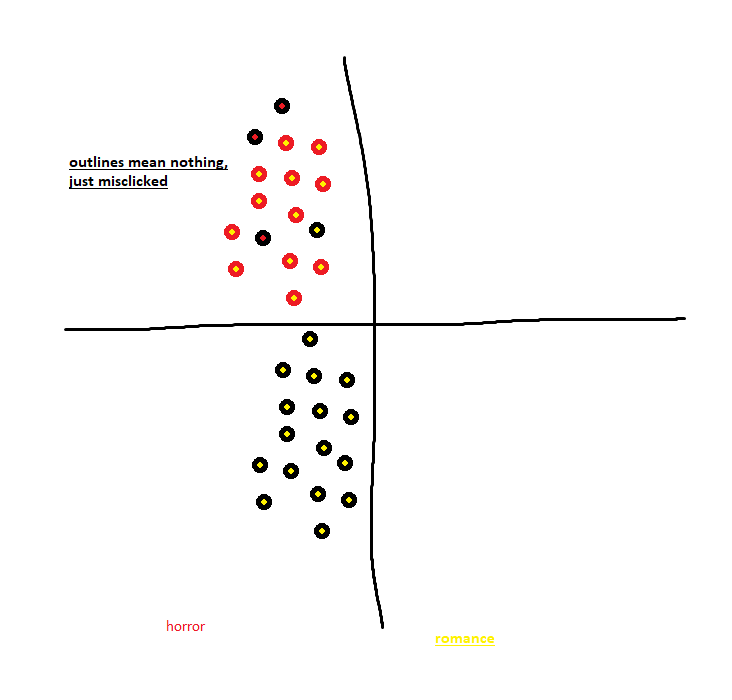
\includegraphics[width=\textwidth]{images/genres_separated.png}
	\centering
	\caption{Original And Converted.}\label{ch3:OrigAndConverted}
\end{figure}

The method to obtain interpretable feature-vectors is an extension of the work by \cite{derracAIJ}. This previous work showed how to, filter out words, cluster words to get features, and obtain rankings of documents on those features. In this section, we further analyse and extend this work, in particular by testing a variety of additional filtering methods and clustering methods, and demonstrating how these feature-vectors can produce simple linear interpretable classifiers. 
%To begin, we filter out terms that will not be well represented in the space, and in-turn will not result in good feature rankings. We do so by first removing all terms below a frequency threshold. Then, for each word we obtain a direction in the space that can induce a ranking of documents on that word, and evaluate how well represented that word is in the space and remove those below a threshold. We can consider the terms remaining to be candidate feature-directions, as they are all well represented in the space and are unlikely to be highly scored as representative due to being infrequent. However, it is possible that they may not represent different information from each other, e.g. "blood" and "bloody" are likely quite similar. Additionally, we can understand that a good feature will not correspond directly to a term, but instead to a more abstract concept, e.g. "Blood, Gore, Horror". To obtain these more abstract feature-directions, and ensure the feature-directions are distinct rather than representing the same information, we cluster together similar feature-directions and obtain their feature-rankings to obtain our final representation. Each of these feature-rankings can be labelled with the cluster of words they are composed of. 



\subsection{Term Rankings}

\noindent \textbf{Structure of a Semantic Space} Salient features of the domain are encoded in the structure of a semantic space, see Section \ref{bg:SemanticSpaces} for more detail. We can expect that for these salient features, they will be more linearly separable than words, and be spatially organized in a way that reflects the similarity between their associated PPMI scores that the space was constructed from. In particular, we expect that documents will be arranged in a direction, where generally the higher the PPMI score for a group of words that correspond to a feature (e.g. $Horror, Scary, Gore$) the further away they will be from those that have low PPMI scores for those words. We give examples of this in Figure \ref{ch3:DirectionsGraphic}, by projecting documents into a 2D space of salient features we are able to show that these documents are structured according to directions for these features. Salient features will typically be a more abstract representation which will be natural in the domain, e.g. in a domain of IMDB movie reviews, genres. However, in this section we show how to extract rankings of documents on words, with the understanding that all words may not be features of the domain. In the next sections, we aim to use these words to extract salient features by filtering and clustering.

\begin{figure}[t]
	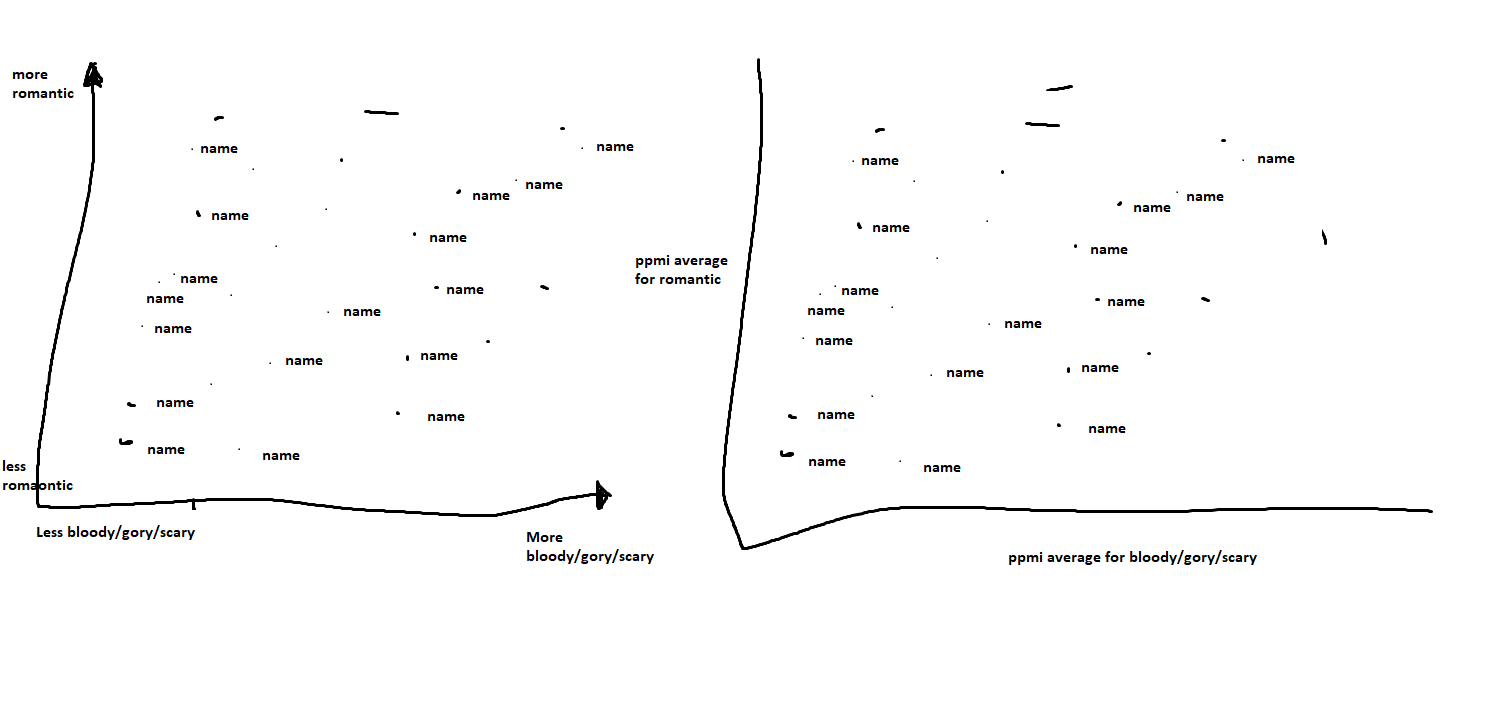
\includegraphics[width=\textwidth]{images/DirectionsGraphic.png}
	\centering
	\caption{Original And Converted.}\label{ch3:DirectionsGraphic}
\end{figure}


\noindent \textbf{Obtaining directions for each word} For each word $w$, a Support Vector Machine (See Section \ref{bg:SVM}) classifier is trained on the binary Bag-Of-Words representation of that word, where words are labelled as positive if they occurred more than once $w_f >= 1$ and negative otherwise. Although the separation of documents is binary, given the structure of the semantic space we can expect for salient features that the documents close to the hyper-plane on the positive side will have lower PPMI scores for the term than those furthest from the hyper-plane on the positive side, as they are closest to the documents that are classified negatively. Following this, we can consider the vector $v_w$ perpendicular to the hyperplane as the direction' that models documents from least relevant at the distance furthest from the hyperplane on the negative side to most relevant for the word $w$ at the distance furthest from the hyperplane at the positive side. In \ref{Figure2a}, we show an example of directions in a toy domain. %Although these directions do formally correspond to vectors, we refer to them as directions to emphasize their intended ordinal meaning: feature directions are aimed at ranking entities rather than e.g.\ measuring degrees of similarity. %Graphical representation of 

\noindent \textbf{Ranking documents on directions} Once we have obtained a direction vector for each word $v_w$ the next step is to quantify the degree to which each document has that word, by obtaining a value that corresponds to how far-up it is on the direction vector. These are our rankings of documents on words, if $p_d$ is the representation of an document in the given vector space as a point then we can think of the dot product between the hyper-plane and the document vector $H_w \cdot p_d$ as the ranking $r_dw$ of the document $d$ for the word $w$, and in particular, we take $r_d1 < r_d2$ to mean that $d_2$ has the property labelled with the word $w$ to a greater extent than $e_1$.  %Graphical representation of entities being ranked on a direction vector

\subsection{Filtering Words}

With the rankings $R_r$, we could create a representation of each document $d$, composed of $w_n$ dimensions, where each dimension is a ranking of the document $d$ on that word $r_dw$. However, many of the words are not spatially important enough in the representation to result in a quality ranking - they are not salient features. In this section, we aim to filter the words that are not separable, we evaluate them using a scoring metric, and remove the words that are not sufficiently well scored. We use three different metrics:

\noindent \textbf{Classification accuracy}. Evaluating the quality in terms of the accuracy of the SVM classifier: if this classifier is sufficiently accurate, it must mean that whether word $w$ relates to document $d$ (i.e.\ whether it is used in the description of $d$) is important enough to affect the semantic space representation of $d$. In such a case, it seems reasonable to assume that $w$ describes a salient property for the given domain.%This is basically copy pasted.
\smallskip

\noindent \textbf{Cohen's Kappa}. One problem with accuracy as a scoring function is that these classification problems are often very imbalanced. In particular, for very rare words, a high accuracy might not necessarily imply that the corresponding direction is accurate. For this reason, X proposed to use Cohen's Kappa score instead. In our experiments, however, we found that accuracy sometimes yields better results, so  as an alternative metric. %This is basically copy pasted.
\smallskip

\noindent \textbf{Normalized Discounted Cumulative Gain} % MATHEMATICS NEEDS TO BE REWRITTEN
This is a standard metric in information retrieval which evaluates the quality of a ranking w.r.t.\ some given relevance scores \cite{jarvelin2002cumulated}.  In our case, the rankings $r_d$ of the document $d$ are those induced by the dot products $v_w \cdot d$ and the relevance scores are determined by the Pointwise Positive Mutual Information (PPMI) score $\textit{ppmi}(w,d)$, of the word $w$ in the BoW representation of entity $d$ where
$\textit{ppmi}(w,d) = \max \big(0, \log\big(\frac{p_{wd}}{p_{w*} \cdotp p_{*d}}\big)\big)$, and
\begin{align*}
p_{wd} &= \frac{n(w, d)}{\sum_{w'} \sum_{d'} n(w', d')}
\end{align*}
where $n(w,d)$ is the number of occurrences of $w$ in the BoW representation of object $d$, $p_{w*} = \sum_{e'} p_{wd'}$ and $p_{*d} = \sum_{w'} p_{w'd}$. %This is basically copy pasted.
\smallskip

By scoring the words on these features, we can apply a simple cut-off (e.g. the top 2000 scored words) to obtain the most salient words. Ideally, this cut-off would be at the point where the words stop corresponding to salient features. However, it is difficult to determine this. In principle, we may expect that accuracy and Kappa are best suited for binary features, as they rely on a hard separation in the space between objects that have the word in their BoW representation and those that do not, while NDCG should be better suited for gradual features. In practice, however, we could not find such a clear pattern in the differences between the words chosen by these metrics despite often finding different words. In Table \ref{Table4}, we show examples of the differences between the largest differences between the scoring methods. % Copy pasted


\subsubsection{Clustering Direction Vectors}

%What are we doing with clustering
If we consider two directions, "Blood" and "Gore", we can understand both of these to be approximating a similar feature of movies, as they both relate to how much blood a movie contains. Because of this, we can expect their directions to be very similar to each other. This is the first idea behind clustering these directions, if we average these directions together we can obtain a direction inbetween them that results in this more abstract feature. As some entities would have the property of being bloody films, but did not necessarily use the term gore in their reviews, same as some entities having the property but using the term gore not bloody, we can understand that this new hyper plane and associated direction more accurately represents the property of a bloody film more than either of the terms individually. By extending this to a clustering method, we can find similar abstract features by ensuring that all similar directions are clustered together. %Similarly, obtaining a hyper plane using a Logistic Regression classifier that uses occurences of both and either of these terms as positive would be similar to this averaged direction.

%What is the value of a cluster label?
The word direction for "beautiful" can be nebulous to the interpreter, as it is not clear what it means for a movie to be ranked highly on 'beautiful'. Considering this, clustering provides another advantage, once we cluster the terms to find the property ("beautiful", "cinematography" "shots") we are given context for the word and more easily intuit the feature, in this case it is a feature about how well the movie was directed. 

The final benefit to clustering the words is that linear classifiers are generally suited better to 'disentangled' representations \cite{Bengio2012}. In this case, we refer to disentanglement in the sense of obtaining a feature vector where each dimension is distinct, rather than the semantic space being naturally clustered. Additionally, if our representation is dense and disentangled into the natural features of the domain, it is unlikely to overfit and will be able to generalize more easily. When investigating the use of directions without clustering in Section \ref{ch3:WordScores} we found that the sparsity of the directions when using only words tends to overfit in simple linear classifiers.

We approach clustering the directions with a variety of methods:

\noindent \textbf{K-Means} K-Means is a clustering algorithm that starts with determining the amount of clusters, $K$. To begin, $K$ centroids $c$ are randomly placed into the space. Then, the distance between each point $p$ and centroid $c$ (in our case, points are determined by rankings) is calculated. Each point $p$ is then assigned to its closest centroid $c$. Then, the centroids are recomputed to be the mean of their assigned points. This process starting with the distance calculation is repeated until the points assigned to the centroids do not change. 
\noindent \textbf{Derrac's K-Means Variation} This is the clustering method used in the previous work \cite{derracAIJ}. As input to the clustering algorithm, we consider the $N$ best-scoring candidate feature directions $v_w$, where $N$ is a hyperparameter. The main idea underlying their approach is to select the cluster centers such that (i) they are among the top-scoring candidate feature directions, and (ii) are as close to being orthogonal to each other as possible. 
 
The output of this step is a set of clusters $C_1,...,C_K$, where we will identify each cluster $C_j$ with a set of words.
We will furthermore write $v_{C_j}$ to denote the centroid of the directions corresponding to the words in the cluster $C_j$, which can be computed as $v_{C_j}= \frac{1}{|C_j|} \sum_{w_l\in C_j} v_l$ provided that the vectors $v_w$ are all normalized. These centroids $v_{C_1},...,v_{C_k}$ are the feature directions that are identified by our method. 



%Although we are able to find the words that are most salient, the properties in the domain may not correspond directly to words. Further, the properties may not be well described by their associated word. In-order to find better representations of properties, we cluster together similar vectors $v_w$, following the assumption that those vectors which are similar are representing some property more general than their individual words, and we can find it between them.
%As the final step, we cluster the best-scoring candidate feature directions $v_w$. Each of these clusters will then define one of the feature directions to be used in applications. The purpose of this clustering step is three-fold: it will ensure that the feature directions are sufficiently different (e.g.\ in a space of movies there is little point in having \emph{funny} and \emph{hilarious} as separate features), it will make the features easier to interpret (as a cluster of terms is more descriptive than an individual term), and it will alleviate sparsity issues when we want to relate features with the BoW representation, which will play an important role for the fine-tuning method described in the next section.


%Table \ref{tabKappaNDCG} displays some examples of clusters that have been obtained for three of the datasets that will be used in the experiments, modelling respectively movies, place-types and newsgroup postings. For each dataset, we used the scoring function that led to the best performance on development data(see Section \ref{secExperiments}). Only the first four words whose direction is closest to the centroid $v_C$ are shown.
%\noindent \textbf{K-Means}
%\noindent \textbf{Derrac's K-Means Variation}
%\noindent \textbf{Mean-shift}
%\noindent \textbf{Hdbscan}

%Our overall aim is to find directions in the semantic space that model salient features of the considered domain. For example, given a semantic space of movies, we would like to find a direction that models the extent to which each movie is scary, among others. Such a direction would then allow us to rank movies from the least scary to the most scary. We will refer to such directions as \emph{feature directions}. Formally, each feature direction will be modelled as a vector $v_f$. However, we refer to \emph{directions} rather than \emph{vectors} to emphasize their intended ordinal meaning: feature directions are aimed at ranking objects rather than e.g.\ measuring degrees of similarity. 
\subsection{Qualitative Results}

\subsubsection{Dimension of the Space}

\subsubsection{Space-type}

\subsubsection{Scoring method}

\subsubsection{Clustering method}

\textbf{The effect of dimensions}


\textbf{The effect of space-type}


\textbf{The effect of scoring method}

\subsection{Quantitative Results}



%Naturally, it is sometimes not enough to see a list of terms and understand the property without domain knowledge. However, by examining how classifiers use these directions to classify key domain knowledge we are better able to understand what they are modelling. For example, when classifying if a movie is a sci-fi, we see that if a movie is ranked highly on the term "science, scientist", then it is not a sci-fi movie. However, when classifying if a movie is a biography, we see that if a movie is ranked highly on "science, scientist" then it is a biography movie. From this, we can understand that the property is not about mad scientists, but normal non-fiction science. 

In this section, we explain the processes to obtain a variety of different Semantic Spaces. \label{ch3:Method}
% Basic explanation of why quantitative results are interesting, valuable, good etc

This section focuses on using linear classifiers to determine how well our method represents domain knowledge compared to standard baselines. We can understand that an accurate representation of domain knowledge will be one that ensures semantically distinct entities are separated, and semantically similar entities are close together. Put another way, if the space is representing domain knowledge well we can expect that the space should be linearly separable for key semantics of the domain. For example, a good vector space in the domain of movies constructed from IMDB movie reviews should contain a natural separation of entities into genres, where Horror movies are spatially distant from Romance movies, and movies that are Romantic Horrors would be somewhere inbetween. We can see an example in Figure \ref{figure:genres_separated}. For a Bag-Of-Words, we can expect similar entities to have similarly scoring terms \ref{PPMI table:PPMI_example}.

\begin{figure}[t]
	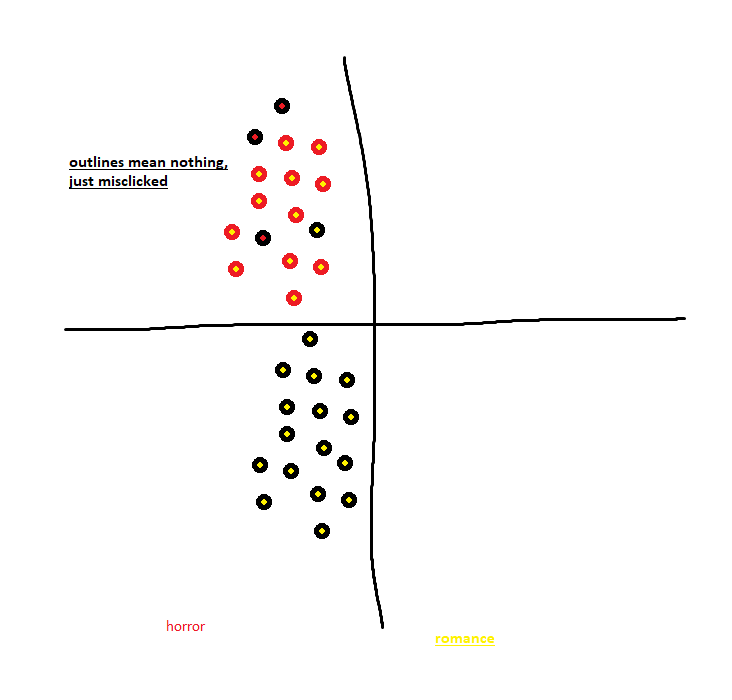
\includegraphics[width=\textwidth]{images/genres_separated.png}
	\centering
	\caption{A conceptual space of movies, where regions correspond to properties and entities are points.}\label{figure:genres_separated}
\end{figure}

\begin{table}[]
	\begin{tabular}{ll}
		& Top PPMI scoring terms                                                \\
		Example Horror Entity      & Term term term term term term term term term term term term term term \\
		Similar Horror Entity      & Term term term term term term term term term term term term term term \\
		Somewhere Inbetween Entity & Term term term term term term term term term term term term term term \\
		Romance Movie              & Term term term term term term term term term term term term term term \\
		Similar Romance movie      & Term term term term term term term term term term term term term term
	\end{tabular}
\caption{Two of the following entities: Those classified as horror, those classified as horror and romance, and those classified as romance with their associated highest value PPMI terms. We show the highest positive instances here as the representation is sparse, even though we can also expect the terms that are low scoring to be similar too.}
\label{table:PPMI_example}
\end{table}

When selecting the parameters to use for the doc2vec space when obtaining directions, we choose the one that scored the highest for its class on a Linear SVM, rather than tuning the entire process around the doc2vecs vectors.
We use the kind of multiclass strategy as a hyper-parameter for each class-type in the grid search. We test the OneVsOne classifier method, treating each as binary problems, the OneVsRest method and the OutputCode method.
We are not able to obtain an MDS space for sentiment or doc2vec spaces for placetypes/movies.

As our work performs well even at lower-depth trees, this gives potential users more flexibility in how they want to present the information, e.g. to a potential client. Compared to bag-of-words, which loses its representation capabilities the lower the depth.

As the newsgroups contained empty documents after removing all words that do not occur in at least 2 documents, we have removed these empty documents, leaving us with 18302 overall documents. Following this, instead of using the train split as determined by previous literature, we did a simple 2/3 train/test split the same as our IMDB dataset.

\subsubsection{Results for vector spaces and bag-of-words}
\begin{table}[]
	\begin{tabular}{llllll}
		& SVM   & DT (N) & DT (3) & DT (2) & DT (1) \\
		PPMI           & 0.594 & \textbf{0.441}  & \textbf{0.44}   & \textbf{0.441}  & \textbf{0.315}  \\
		PCA 50         & 0.509 & 0.418  & 0.308  & 0.418  & 0.229  \\
		PCA 100        & 0.577 & 0.412  & 0.36   & 0.412  & 0.238  \\
		PCA 200        & 0.597 & 0.409  & 0.342  & 0.409  & 0.24   \\
		D2V 50         & 0.592 & 0.308  & 0.308  & 0.308  & 0.244  \\
		D2V 100        & 0.613 & 0.335  & 0.324  & 0.335  & 0.234  \\
		D2V 200        & \textbf{0.619} & 0.369  & 0.369  & 0.369  & 0.251  \\
		AWV 50         & 0.348 & 0.233  & 0.233  & 0.233  & 0.213  \\
		AWV 100        & 0.378 & 0.236  & 0.236  & 0.236  & 0.208  \\
		AWV 200        & 0.451 & 0.236  & 0.236  & 0.236  & 0.22   \\
		MDS 50         & 0.381 & 0.242  & 0.242  & 0.242  & 0.191  \\
		MDS 100        & 0.432 & 0.238  & 0.238  & 0.238  & 0.148  \\
		MDS 200        & 0.481 & 0.243  & 0.243  & 0.243  & 0.188 
	\end{tabular}
	\caption{Results for 20 newsgroups (Original table F1 scores only).}
	\label{table:Newsgroups}
\end{table}

\begin{table}[]
\begin{tabular}{llllll}
	& avg\_acc    & avg\_f1     & avg\_kappa  & avg\_prec   & avg\_recall \\
	PCA 50  & 0.96490308  & 0.492247891 & 0.457299224 & 0.711658333 & 0.376247516 \\
	AWV 50  & 0.836962294 & 0.348019806 & 0.287991958 & 0.221993012 & 0.805053757 \\
	MDS 50  & 0.850165959 & 0.380514451 & 0.319361959 & 0.249390206 & 0.80239975  \\
	D2V 50  & 0.969251195 & 0.583050235 & 0.552867243 & 0.762328571 & 0.472039711 \\
	PCA 100 & 0.96798991  & 0.573312826 & 0.548472358 & 0.76084381  & 0.45994634  \\
	AWV 100 & 0.8581718   & 0.37842844  & 0.32249064  & 0.247582046 & 0.802600456 \\
	MDS 100 & 0.877734997 & 0.431782978 & 0.367431954 & 0.304064453 & 0.744501764 \\
	D2V 100 & 0.969576474 & 0.607208735 & 0.580914149 & 0.763888161 & 0.503862585 \\
	PCA 200 & 0.96814923  & 0.600195646 & 0.579020555 & 0.736568432 & 0.506431769 \\
	AWV 200 & 0.960010621 & 0.451033454 & 0.417523124 & 0.628312372 & 0.351778753 \\
	MDS 200 & 0.964630908 & 0.480837639 & 0.450593914 & 0.789387894 & 0.345709284 \\
	D2V 200 & 0.969138343 & 0.619296679 & 0.597329654 & 0.731193811 & 0.537102079
\end{tabular}
	\caption{Results for 20 newsgroups SVM.}
	\label{table:Newsgroups}
\end{table}

\begin{table}[]
	\begin{tabular}{llll}
		& F1          & PREC        & RECALL      \\
		PCA 50  & 0.328304254 & 0.206683241 & 0.797709964 \\
		AWV 50  & 0.232797129 & 0.136574918 & 0.787908695 \\
		MDS 50  & 0.242237348 & 0.144618794 & 0.745359468 \\
		D2V 50  & 0.262485129 & 0.159552724 & 0.739667629 \\
		PCA 100 & 0.348355036 & 0.590710997 & 0.247011539 \\
		AWV 100 & 0.236469254 & 0.139836252 & 0.765381631 \\
		MDS 100 & 0.237535645 & 0.140254022 & 0.775272724 \\
		D2V 100 & 0.241880243 & 0.144911904 & 0.731095552 \\
		PCA 200 & 0.360425936 & 0.540033963 & 0.270470942 \\
		AWV 200 & 0.235578784 & 0.139287267 & 0.763171354 \\
		MDS 200 & 0.243002892 & 0.145997046 & 0.72416485  \\
		D2V 200 & 0.242582271 & 0.144063637 & 0.767313249
	\end{tabular}
	\caption{Results for 20 newsgroups DT3.}
	\label{table:Newsgroups}
\end{table}

\begin{table}[]
	\begin{tabular}{llll}
		& F1          & PREC        & RECALL      \\
		PCA 50  & 0.351456416 & 0.23188865  & 0.725588605 \\
		AWV 50  & 0.277555185 & 0.175212293 & 0.667373129 \\
		MDS 50  & 0.262512227 & 0.160257903 & 0.725294194 \\
		D2V 50  & 0.291764949 & 0.1910914   & 0.616623507 \\
		PCA 100 & 0.36290335  & 0.24352329  & 0.711882698 \\
		AWV 100 & 0.260604694 & 0.160646408 & 0.689841882 \\
		MDS 100 & 0.262095206 & 0.161124391 & 0.70203524  \\
		D2V 100 & 0.275263826 & 0.173804325 & 0.661305683 \\
		PCA 200 & 0.359230759 & 0.239547295 & 0.717920958 \\
		AWV 200 & 0.249564678 & 0.151789776 & 0.701313625 \\
		MDS 200 & 0.253938183 & 0.153568133 & 0.733049213 \\
		D2V 200 & 0.273966602 & 0.175932631 & 0.618748321
	\end{tabular}
	\caption{Results for 20 newsgroups DT2.}
	\label{table:Newsgroups}
\end{table}

\begin{table}[]
	\begin{tabular}{llll}
		& F1          & PREC        & RECALL      \\
		PCA 50  & 0.237796799 & 0.139329768 & 0.810816271 \\
		AWV 50  & 0.212916931 & 0.123466917 & 0.772798069 \\
		MDS 50  & 0.174946697 & 0.099635471 & 0.716605845 \\
		D2V 50  & 0.206890545 & 0.119473856 & 0.771060354 \\
		PCA 100 & 0.241437752 & 0.142104023 & 0.80217534  \\
		AWV 100 & 0.208197142 & 0.1202674   & 0.774308646 \\
		MDS 100 & 0.186613434 & 0.105176833 & 0.826757278 \\
		D2V 100 & 0.196855298 & 0.112987628 & 0.76381335  \\
		PCA 200 & 0.24018672  & 0.140977055 & 0.810699841 \\
		AWV 200 & 0.220189174 & 0.128863697 & 0.755880029 \\
		MDS 200 & 0.187525181 & 0.105846321 & 0.821304769 \\
		D2V 200 & 0.207592806 & 0.121252635 & 0.72097962 
	\end{tabular}
	\caption{Results for 20 newsgroups DT1.}
	\label{table:Newsgroups}
\end{table}


\begin{table}[]
	\begin{tabular}{llll}
		& F1          & PREC        & RECALL      \\
		PCA 50  & 0.41928432  & 0.405469685 & 0.434073508 \\
		AWV 50  & 0.30215353  & 0.281684719 & 0.325830202 \\
		MDS 50  & 0.293534597 & 0.279429073 & 0.309139919 \\
		D2V 50  & 0.38212279  & 0.396860235 & 0.368440707 \\
		PCA 100 & 0.41444605  & 0.39177829  & 0.439897947 \\
		AWV 100 & 0.296573651 & 0.277583826 & 0.318352508 \\
		MDS 100 & 0.303315524 & 0.284560799 & 0.324716839 \\
		D2V 100 & 0.369399726 & 0.390914592 & 0.350129557 \\
		PCA 200 & 0.405630591 & 0.384607892 & 0.429084378 \\
		AWV 200 & 0.307071322 & 0.287564233 & 0.329417555 \\
		MDS 200 & 0.295333334 & 0.275822911 & 0.31781401  \\
		D2V 200 & 0.350219973 & 0.37188488  & 0.330940371
	\end{tabular}
	\caption{Results for 20 newsgroups DTN.}
	\label{table:Newsgroups}
\end{table}

\begin{table}[]
	\begin{tabular}{llll}
		& F1          & Precision   & Recall  \\
		PCA 50  & 0.886155063 & 0.876447574 & 0.89608 \\
		AWV 50  & 0.755943328 & 0.756367131 & 0.75552 \\
		D2V 50  & 0.86072602  & 0.862176914 & 0.85928 \\
		PCA 100 & 0.891788242 & 0.881575862 & 0.90224 \\
		AWV 100 & 0.801005145 & 0.798743139 & 0.80328 \\
		D2V 100 & 0.872537705 & 0.8680814   & 0.87704 \\
		PCA 200 & 0.892751333 & 0.881779165 & 0.904   \\
		AWV 200 & 0.828502127 & 0.823622421 & 0.83344 \\
		D2V 200 & 0.878093492 & 0.874851108 & 0.88136
	\end{tabular}
	\caption{Results for Sentiment SVM.}
	\label{table:Newsgroups}
\end{table}

\begin{table}[]
	\begin{tabular}{llll}
		& avg\_f1     & avg\_prec   & avg\_recall \\
		PPMI    & 0.699599048 & 0.574907331 & 0.89336     \\
		PCA 50  & 0.124525871 & 0.590631365 & 0.0696      \\
		AWV 50  & 0.495850524 & 0.608827297 & 0.41824     \\
		D2V 50  & 0.664416948 & 0.625264644 & 0.7088      \\
		PCA 100 & 0.705496839 & 0.8337515   & 0.61144     \\
		AWV 100 & 0.599821349 & 0.678968655 & 0.5372      \\
		D2V 100 & 0.629258374 & 0.567823344 & 0.7056      \\
		PCA 200 & 0.705458908 & 0.833496892 & 0.61152     \\
		AWV 200 & 0.651572425 & 0.63521009  & 0.6688      \\
		D2V 200 & 0.663735313 & 0.603961695 & 0.73664    
	\end{tabular}
	\caption{Results for Sentiment DT1.}
	\label{table:Newsgroups}
\end{table}

\begin{table}[]
	\begin{tabular}{llll}
		& F1          & PREC        & RECALL  \\
		PPMI    & 0.718834534 & 0.606500577 & 0.88224 \\
		PCA 50  & 0.769670528 & 0.72629188  & 0.81856 \\
		AWV 50  & 0.621045392 & 0.594426565 & 0.65016 \\
		D2V 50  & 0.708094413 & 0.606995885 & 0.8496  \\
		PCA 100 & 0.769658907 & 0.726208218 & 0.81864 \\
		AWV 100 & 0.693895748 & 0.607262905 & 0.80936 \\
		D2V 100 & 0.707420276 & 0.620556461 & 0.82256 \\
		PCA 200 & 0.769572084 & 0.72605364  & 0.81864 \\
		AWV 200 & 0.663435963 & 0.609166945 & 0.72832 \\
		D2V 200 & 0.694119925 & 0.581737531 & 0.86032
	\end{tabular}
	\caption{Results for Sentiment DT2.}
	\label{table:Newsgroups}
\end{table}

\begin{table}[]
	\begin{tabular}{llll}
		& F1          & PREC        & RECALL  \\
		PPMI    & 0.730120722 & 0.624793671 & 0.87816 \\
		PCA 50  & 0.773241796 & 0.790326623 & 0.75688 \\
		AWV 50  & 0.716599792 & 0.668978912 & 0.77152 \\
		D2V 50  & 0.706911296 & 0.687509451 & 0.72744 \\
		PCA 100 & 0.773228733 & 0.790212126 & 0.75696 \\
		AWV 100 & 0.651385973 & 0.701226824 & 0.60816 \\
		D2V 100 & 0.724228567 & 0.658482289 & 0.80456 \\
		PCA 200 & 0.773133962 & 0.790014194 & 0.75696 \\
		AWV 200 & 0.686097207 & 0.692470665 & 0.67984 \\
		D2V 200 & 0.688555129 & 0.668651541 & 0.70968
	\end{tabular}
	\caption{Results for Sentiment DT3.}
	\label{table:Newsgroups}
\end{table}

\begin{table}[]
	\begin{tabular}{llll}
		& F1          & PREC        & RECALL  \\
		PPMI    & 0.709744995 & 0.714842165 & 0.70472 \\
		PCA 50  & 0.778979658 & 0.786086673 & 0.772   \\
		AWV 50  & 0.645669922 & 0.645980141 & 0.64536 \\
		D2V 50  & 0.699698128 & 0.704090725 & 0.69536 \\
		PCA 100 & 0.773306533 & 0.777212121 & 0.76944 \\
		AWV 100 & 0.647586262 & 0.648053197 & 0.64712 \\
		D2V 100 & 0.683666547 & 0.682060674 & 0.68528 \\
		PCA 200 & 0.770502991 & 0.773265651 & 0.76776 \\
		AWV 200 & 0.663097363 & 0.657491152 & 0.6688  \\
		D2V 200 & 0.665625    & 0.666693419 & 0.66456
	\end{tabular}
	\caption{Results for Sentiment DTN.}
	\label{table:Newsgroups}
\end{table}

\begin{table}[]
	\begin{tabular}{llllll}
		& avg\_acc    & avg\_f1     & avg\_kappa  & avg\_prec   & avg\_recall \\
		PCA 50  & 0.803602223 & 0.443589681 & 0.308199143 & 0.339736332 & 0.638891067 \\
		AWV 50  & 0.810116881 & 0.457499286 & 0.323892593 & 0.349551692 & 0.661907853 \\
		MDS 50  & 0.813565817 & 0.457003603 & 0.323002846 & 0.364634555 & 0.61204707  \\
		PCA 100 & 0.821421728 & 0.450122408 & 0.32121053  & 0.35527646  & 0.614052074 \\
		AWV 100 & 0.835409082 & 0.455127069 & 0.336542753 & 0.364636358 & 0.6053566   \\
		MDS 100 & 0.83713355  & 0.474728943 & 0.352474877 & 0.393159213 & 0.599006284 \\
		PCA 200 & 0.84671393  & 0.474074812 & 0.360353916 & 0.395372385 & 0.591897289 \\
		AWV 200 & 0.849971259 & 0.465697168 & 0.355000122 & 0.385607296 & 0.587777361 \\
		MDS 200 & 0.861084499 & 0.476306142 & 0.367476644 & 0.425416709 & 0.541024925
	\end{tabular}
	\caption{Results for OpenCYC SVM.}
	\label{table:Newsgroups}
\end{table}

\begin{table}[]
	\begin{tabular}{llllll}
		& avg\_acc    & avg\_f1     & avg\_kappa  & avg\_prec   & avg\_recall \\
		PCA 50  & 0.695152328 & 0.341785127 & 0.157118987 & 0.242841085 & 0.576797613 \\
		AWV 50  & 0.728300441 & 0.39586446  & 0.226931085 & 0.281210223 & 0.668370655 \\
		MDS 50  & 0.728492048 & 0.361747133 & 0.19053657  & 0.26813119  & 0.555800661 \\
		PCA 100 & 0.646100786 & 0.305716926 & 0.103702685 & 0.214560016 & 0.531547629 \\
		AWV 100 & 0.69898448  & 0.352968414 & 0.174088352 & 0.251372807 & 0.592390968 \\
		MDS 100 & 0.722552213 & 0.355478522 & 0.17636028  & 0.262349467 & 0.551113186 \\
		PCA 200 & 0.715845947 & 0.333121225 & 0.153256681 & 0.245505135 & 0.517977489 \\
		AWV 200 & 0.760682123 & 0.382249254 & 0.221321346 & 0.282220454 & 0.592115806 \\
		MDS 200 & 0.730599732 & 0.374349802 & 0.195944453 & 0.279258101 & 0.567639997
	\end{tabular}
	\caption{Results for OpenCYC DT3.}
	\label{table:Newsgroups}
\end{table}

\begin{table}[]
	\begin{tabular}{llllll}
		& avg\_acc    & avg\_f1     & avg\_kappa  & avg\_prec   & avg\_recall \\
		PCA 50  & 0.707606821 & 0.343429484 & 0.156929616 & 0.251027506 & 0.543482807 \\
		AWV 50  & 0.650890975 & 0.375734032 & 0.183056015 & 0.256467865 & 0.702350672 \\
		MDS 50  & 0.707415214 & 0.387617362 & 0.194958449 & 0.275974626 & 0.650954337 \\
		PCA 100 & 0.623107875 & 0.310355155 & 0.102113833 & 0.208258091 & 0.608829572 \\
		AWV 100 & 0.689020885 & 0.366415742 & 0.181031062 & 0.258842906 & 0.626985335 \\
		MDS 100 & 0.694002683 & 0.369986155 & 0.180288011 & 0.265420819 & 0.610498481 \\
		PCA 200 & 0.689020885 & 0.333046463 & 0.147294515 & 0.245169324 & 0.519115278 \\
		AWV 200 & 0.646292393 & 0.325676238 & 0.128022927 & 0.234108504 & 0.534889609 \\
		MDS 200 & 0.700134125 & 0.397197263 & 0.204265502 & 0.294908338 & 0.608125541
	\end{tabular}
	\caption{Results for OpenCYC DT2.}
	\label{table:Newsgroups}
\end{table}

\begin{table}[]
	\begin{tabular}{llllll}
		& avg\_acc    & avg\_f1     & avg\_kappa  & avg\_prec   & avg\_recall \\
		PCA 50  & 0.553745928 & 0.310633902 & 0.092680202 & 0.206504902 & 0.626587132 \\
		AWV 50  & 0.624640736 & 0.382961496 & 0.17878069  & 0.262022566 & 0.711241624 \\
		MDS 50  & 0.615443572 & 0.35823563  & 0.146293722 & 0.240950353 & 0.697990127 \\
		PCA 100 & 0.585744395 & 0.346181476 & 0.13321519  & 0.228755781 & 0.711317277 \\
		AWV 100 & 0.620042154 & 0.380088459 & 0.176711823 & 0.254076387 & 0.754085962 \\
		MDS 100 & 0.624065913 & 0.364362146 & 0.155358843 & 0.245217405 & 0.708701922 \\
		PCA 200 & 0.601073002 & 0.344834471 & 0.134633794 & 0.229762238 & 0.690818169 \\
		AWV 200 & 0.643993102 & 0.349374827 & 0.146997089 & 0.236040865 & 0.672062735 \\
		MDS 200 & 0.597049243 & 0.358243938 & 0.143631945 & 0.237385589 & 0.729803158
	\end{tabular}
	\caption{Results for OpenCYC DT1.}
	\label{table:Newsgroups}
\end{table}


\begin{table}[]
	\begin{tabular}{llllll}
		& avg\_acc    & avg\_f1     & avg\_kappa  & avg\_prec   & avg\_recall \\
		PCA 50  & 0.831960146 & 0.297281859 & 0.174312986 & 0.284553476 & 0.311202271 \\
		AWV 50  & 0.843839816 & 0.361596554 & 0.244157721 & 0.335722254 & 0.391792196 \\
		MDS 50  & 0.842690171 & 0.305261263 & 0.187421961 & 0.319838245 & 0.291955087 \\
		PCA 100 & 0.831768538 & 0.308890047 & 0.18386471  & 0.311999386 & 0.30584207  \\
		AWV 100 & 0.825828703 & 0.3157161   & 0.187815304 & 0.299946267 & 0.333236166 \\
		MDS 100 & 0.826403526 & 0.29890705  & 0.170454934 & 0.273414301 & 0.329642427 \\
		PCA 200 & 0.829852462 & 0.283509252 & 0.157446109 & 0.285790467 & 0.281264167 \\
		AWV 200 & 0.825062272 & 0.315853073 & 0.187303114 & 0.28455479  & 0.354887247 \\
		MDS 200 & 0.826211918 & 0.257117269 & 0.118759787 & 0.273406638 & 0.242659775
	\end{tabular}
	\caption{Results for OpenCYC DTN.}
	\label{table:Newsgroups}
\end{table}

\begin{table}[]
	\begin{tabular}{llllll}
		& avg\_acc    & avg\_f1     & avg\_kappa  & avg\_prec   & avg\_recall \\
		PCA 50  & 0.895572264 & 0.568015809 & 0.501678075 & 0.487221026 & 0.680933505 \\
		AWV 50  & 0.932330827 & 0.54620429  & 0.499671391 & 0.626786958 & 0.483981376 \\
		MDS 50  & 0.908103592 & 0.586608962 & 0.515425669 & 0.512247438 & 0.686226545 \\
		PCA 100 & 0.923141186 & 0.558970742 & 0.491390942 & 0.619275607 & 0.509368588 \\
		AWV 100 & 0.94235589  & 0.594804035 & 0.555653205 & 0.668948188 & 0.53545577  \\
		MDS 100 & 0.926482874 & 0.615292664 & 0.557389577 & 0.580419711 & 0.654623981 \\
		PCA 200 & 0.917293233 & 0.541635593 & 0.475003669 & 0.618051665 & 0.482036476 \\
		AWV 200 & 0.923141186 & 0.621747387 & 0.572616698 & 0.588166472 & 0.659395043 \\
		MDS 200 & 0.932330827 & 0.619167077 & 0.553015718 & 0.617480101 & 0.620863297
	\end{tabular}
	\caption{Results for Foursquare SVM.}
	\label{table:Newsgroups}
\end{table}

\begin{table}[]
\begin{tabular}{llllll}
	& avg\_acc    & avg\_f1     & avg\_kappa  & avg\_prec   & avg\_recall \\
	PCA 50  & 0.839598997 & 0.372257009 & 0.267318657 & 0.30580459  & 0.475608395 \\
	AWV 50  & 0.888888889 & 0.333089916 & 0.248206274 & 0.405456349 & 0.282643327 \\
	MDS 50  & 0.830409357 & 0.419208689 & 0.316494416 & 0.342341941 & 0.540588045 \\
	PCA 100 & 0.868838764 & 0.258742227 & 0.169002156 & 0.285630499 & 0.236480745 \\
	AWV 100 & 0.850459482 & 0.452009868 & 0.353271904 & 0.375570892 & 0.567514666 \\
	MDS 100 & 0.898913952 & 0.420948186 & 0.345823805 & 0.424938272 & 0.417032335 \\
	PCA 200 & 0.860484545 & 0.388032162 & 0.296331387 & 0.327684978 & 0.475624149 \\
	AWV 200 & 0.83625731  & 0.398606427 & 0.303172463 & 0.311572257 & 0.553111974 \\
	MDS 200 & 0.859649123 & 0.453720532 & 0.367624409 & 0.396116154 & 0.530929926
\end{tabular}
\caption{Results for Foursquare DT3.}
\label{table:Newsgroups}
\end{table}

\begin{table}[]
\begin{tabular}{llllll}
	& avg\_acc    & avg\_f1     & avg\_kappa  & avg\_prec   & avg\_recall \\
	PCA 50  & 0.82289056  & 0.392580599 & 0.281920837 & 0.309401801 & 0.536926586 \\
	AWV 50  & 0.827903091 & 0.478278996 & 0.381606764 & 0.36842967  & 0.681460044 \\
	MDS 50  & 0.822055138 & 0.424355448 & 0.308763351 & 0.361969434 & 0.512724306 \\
	PCA 100 & 0.755221387 & 0.296725552 & 0.167952229 & 0.209764361 & 0.50684722  \\
	AWV 100 & 0.904761905 & 0.389295248 & 0.325049447 & 0.490226337 & 0.322829039 \\
	MDS 100 & 0.897243108 & 0.409821491 & 0.332196168 & 0.46487494  & 0.366426887 \\
	PCA 200 & 0.730994152 & 0.307534481 & 0.177887091 & 0.232183759 & 0.455289988 \\
	AWV 200 & 0.857978279 & 0.468783935 & 0.385734234 & 0.391391941 & 0.584325748 \\
	MDS 200 & 0.803675856 & 0.42673129  & 0.312371899 & 0.342173461 & 0.56679838 
\end{tabular}
\caption{Results for Foursquare DT2.}
\label{table:Newsgroups}
\end{table}

\begin{table}[]
\begin{tabular}{llllll}
	& avg\_acc    & avg\_f1     & avg\_kappa  & avg\_prec   & avg\_recall \\
	PCA 50  & 0.662489557 & 0.229077055 & 0.079211523 & 0.147644224 & 0.510816983 \\
	AWV 50  & 0.722639933 & 0.396225837 & 0.275700337 & 0.282063751 & 0.665633342 \\
	MDS 50  & 0.521303258 & 0.260605438 & 0.090701456 & 0.161991543 & 0.66610041  \\
	PCA 100 & 0.746867168 & 0.323216815 & 0.186288095 & 0.231022684 & 0.537860651 \\
	AWV 100 & 0.766917293 & 0.401290958 & 0.288812617 & 0.277038046 & 0.727641889 \\
	MDS 100 & 0.914786967 & 0.437858477 & 0.374376011 & 0.500864198 & 0.388933027 \\
	PCA 200 & 0.730994152 & 0.342263034 & 0.202224854 & 0.240331095 & 0.594342133 \\
	AWV 200 & 0.746031746 & 0.380859893 & 0.262290616 & 0.266223919 & 0.668879135 \\
	MDS 200 & 0.732664996 & 0.371307214 & 0.226238672 & 0.267356477 & 0.607514701
\end{tabular}
\caption{Results for Foursquare DT1.}
\label{table:Newsgroups}
\end{table}

\begin{table}[]
\begin{tabular}{llllll}
	& avg\_acc    & avg\_f1     & avg\_kappa  & avg\_prec   & avg\_recall \\
	PCA 50  & 0.887218045 & 0.398256756 & 0.320725011 & 0.395149528 & 0.401413239 \\
	AWV 50  & 0.904761905 & 0.505069034 & 0.438593015 & 0.518028604 & 0.49274206  \\
	MDS 50  & 0.89390142  & 0.39499897  & 0.323143947 & 0.395981215 & 0.394021585 \\
	PCA 100 & 0.873015873 & 0.376756341 & 0.289354017 & 0.400611698 & 0.355582361 \\
	AWV 100 & 0.884711779 & 0.35844367  & 0.268995105 & 0.400944522 & 0.324089582 \\
	MDS 100 & 0.854636591 & 0.377612135 & 0.283423014 & 0.321749605 & 0.456947953 \\
	PCA 200 & 0.874686717 & 0.326303504 & 0.247282108 & 0.342929273 & 0.311215282 \\
	AWV 200 & 0.886382623 & 0.395980062 & 0.303883209 & 0.44741453  & 0.355152029 \\
	MDS 200 & 0.893065998 & 0.461813202 & 0.392690903 & 0.471080118 & 0.452903843
\end{tabular}
\caption{Results for Foursquare DTN.}
\label{table:Newsgroups}
\end{table}

\begin{table}[]
	\begin{tabular}{llllll}
		& avg\_acc    & avg\_f1     & avg\_kappa  & avg\_prec   & avg\_recall \\
		PCA 50  & 0.810559006 & 0.358148107 & 0.234048804 & 0.299351526 & 0.44568688  \\
		AWV 50  & 0.836438923 & 0.451222703 & 0.336497634 & 0.374448235 & 0.567599713 \\
		MDS 50  & 0.784679089 & 0.392395666 & 0.24443375  & 0.313753839 & 0.523646773 \\
		PCA 100 & 0.824016563 & 0.361529188 & 0.239800468 & 0.316458032 & 0.421570923 \\
		AWV 100 & 0.867494824 & 0.513755413 & 0.413110212 & 0.434108709 & 0.629194937 \\
		MDS 100 & 0.713250518 & 0.390532004 & 0.227207011 & 0.280588887 & 0.642142724 \\
		PCA 200 & 0.8436853   & 0.40092042  & 0.291657581 & 0.35733735  & 0.456611589 \\
		AWV 200 & 0.865424431 & 0.513988009 & 0.41302185  & 0.445389498 & 0.60756459  \\
		MDS 200 & 0.637681159 & 0.39650034  & 0.213717085 & 0.262253502 & 0.812329599
	\end{tabular}
	\caption{Results for Geonames SVM.}
	\label{table:Newsgroups}
\end{table}

\begin{table}[]
\begin{tabular}{llllll}
	& avg\_acc    & avg\_f1     & avg\_kappa  & avg\_prec   & avg\_recall \\
	PCA 50  & 0.680124224 & 0.29478471  & 0.122501925 & 0.201991012 & 0.545286876 \\
	AWV 50  & 0.713250518 & 0.25377     & 0.100391576 & 0.183142726 & 0.413064417 \\
	MDS 50  & 0.784679089 & 0.261891846 & 0.136012091 & 0.2084956   & 0.352053677 \\
	PCA 100 & 0.841614907 & 0.237260066 & 0.130180867 & 0.284786642 & 0.203327746 \\
	AWV 100 & 0.755693582 & 0.365164916 & 0.192834906 & 0.305374281 & 0.454069216 \\
	MDS 100 & 0.607660455 & 0.227454345 & 0.032886481 & 0.167615777 & 0.353738392 \\
	PCA 200 & 0.680124224 & 0.189278463 & 0.003823489 & 0.133089599 & 0.327578072 \\
	AWV 200 & 0.841614907 & 0.367019639 & 0.249986812 & 0.373118265 & 0.361117172 \\
	MDS 200 & 0.796066253 & 0.271625693 & 0.134331393 & 0.24476518  & 0.305108249
\end{tabular}
\caption{Results for Geonames DT3.}
\label{table:Newsgroups}
\end{table}

\begin{table}[]
\begin{tabular}{llllll}
	& avg\_acc    & avg\_f1     & avg\_kappa  & avg\_prec   & avg\_recall \\
	PCA 50  & 0.69047619  & 0.305148854 & 0.130369825 & 0.21577343  & 0.520918146 \\
	AWV 50  & 0.738095238 & 0.310954829 & 0.15490415  & 0.238367125 & 0.447108622 \\
	MDS 50  & 0.694616977 & 0.33974778  & 0.159514116 & 0.2446167   & 0.555959698 \\
	PCA 100 & 0.67805383  & 0.237734434 & 0.065010282 & 0.164848865 & 0.426151008 \\
	AWV 100 & 0.754658385 & 0.323247726 & 0.176195969 & 0.247133088 & 0.467114564 \\
	MDS 100 & 0.531055901 & 0.24795975  & 0.02750648  & 0.163433649 & 0.513575287 \\
	PCA 200 & 0.6563147   & 0.259807247 & 0.073980668 & 0.178667481 & 0.475958102 \\
	AWV 200 & 0.85300207  & 0.173697283 & 0.090449158 & 0.20356175  & 0.151474514 \\
	MDS 200 & 0.667701863 & 0.229791347 & 0.036946057 & 0.151458025 & 0.475950563
\end{tabular}
\caption{Results for Geonames DT2.}
\label{table:Newsgroups}
\end{table}

\begin{table}[]
\begin{tabular}{llllll}
	& avg\_acc    & avg\_f1     & avg\_kappa  & avg\_prec   & avg\_recall \\
	PCA 50  & 0.502070393 & 0.301104799 & 0.061819352 & 0.198359173 & 0.624669842 \\
	AWV 50  & 0.660455487 & 0.313961336 & 0.134392586 & 0.224578492 & 0.521532785 \\
	MDS 50  & 0.626293996 & 0.349125673 & 0.147011085 & 0.243137775 & 0.61892611  \\
	PCA 100 & 0.594202899 & 0.291992239 & 0.100440755 & 0.191654145 & 0.612833373 \\
	AWV 100 & 0.657349896 & 0.325658374 & 0.14728302  & 0.235431725 & 0.528013996 \\
	MDS 100 & 0.553830228 & 0.297616636 & 0.058027099 & 0.206694373 & 0.531351498 \\
	PCA 200 & 0.602484472 & 0.285530102 & 0.095389029 & 0.190597186 & 0.568877329 \\
	AWV 200 & 0.593167702 & 0.308568052 & 0.105417935 & 0.203284664 & 0.640064657 \\
	MDS 200 & 0.685300207 & 0.272314442 & 0.093166554 & 0.218701726 & 0.360748654
\end{tabular}
\caption{Results for Geonames DT1.}
\label{table:Newsgroups}
\end{table}

\begin{table}[]
\begin{tabular}{llllll}
	& avg\_acc    & avg\_f1     & avg\_kappa  & avg\_prec   & avg\_recall \\
	PCA 50  & 0.81884058  & 0.206287264 & 0.089323711 & 0.196516538 & 0.217080418 \\
	AWV 50  & 0.83126294  & 0.257954417 & 0.149132237 & 0.24187974  & 0.27631775  \\
	MDS 50  & 0.803312629 & 0.265083269 & 0.11955942  & 0.268740939 & 0.261523827 \\
	PCA 100 & 0.820910973 & 0.24285113  & 0.10287381  & 0.286105247 & 0.210957969 \\
	AWV 100 & 0.845755694 & 0.274948597 & 0.176276415 & 0.27827957  & 0.271696423 \\
	MDS 100 & 0.82815735  & 0.194417219 & 0.088608744 & 0.182779779 & 0.207637318 \\
	PCA 200 & 0.801242236 & 0.239213047 & 0.101080713 & 0.230680272 & 0.248401316 \\
	AWV 200 & 0.8126294   & 0.332311235 & 0.192696161 & 0.296749178 & 0.377557229 \\
	MDS 200 & 0.844720497 & 0.294533825 & 0.15434765  & 0.380248649 & 0.240353795
\end{tabular}
\caption{Results for Geonames DTN.}
\label{table:Newsgroups}
\end{table}

\begin{table}[]
	
	\caption{Results for Genres SVM.}
	\label{table:Newsgroups}
\end{table}

\begin{table}[]

\caption{Results for Genres DT3.}
\label{table:Newsgroups}
\end{table}

\begin{table}[]

\caption{Results for Genres DT2.}
\label{table:Newsgroups}
\end{table}

\begin{table}[]

\caption{Results for Genres DT1.}
\label{table:Newsgroups}
\end{table}

\begin{table}[]

\caption{Results for Genres DTN.}
\label{table:Newsgroups}
\end{table}

\begin{table}[]
	
	\caption{Results for Keywords SVM.}
	\label{table:Newsgroups}
\end{table}

\begin{table}[]

\caption{Results for Keywords DT3.}
\label{table:Newsgroups}
\end{table}

\begin{table}[]

\caption{Results for Keywords DT2.}
\label{table:Newsgroups}
\end{table}

\begin{table}[]

\caption{Results for Keywords DT1.}
\label{table:Newsgroups}
\end{table}

\begin{table}[]

\caption{Results for Keywords DTN.}
\label{table:Newsgroups}
\end{table}

\begin{table}[]
	
	\caption{Results for Ratings SVM.}
	\label{table:Newsgroups}
\end{table}

\begin{table}[]

\caption{Results for Ratings DT3.}
\label{table:Newsgroups}
\end{table}

\begin{table}[]

\caption{Results for Ratings DT2.}
\label{table:Newsgroups}
\end{table}

\begin{table}[]

\caption{Results for Ratings DT1.}
\label{table:Newsgroups}
\end{table}

\begin{table}[]

\caption{Results for Ratings DTN.}
\label{table:Newsgroups}
\end{table}

% Deeper explanation of our methodology and approach

\subsection{Interpretability Results}
